\chapter{Background Theory}
\label{BackgroundTheory}
\graphicspath{{Figures/BackgroundTheory/}{Figures/Common/}}

\section{Phase-space methods}
\label{BackgroundTheory:PhaseSpaceMethods}
%Focus primarily on truncated Wigner.

\section{Absorbing boundary layers for Schrödinger-type equations}
\label{BackgroundTheory:AbsorbingBoundaryLayers}


To solve any partial differential equation numerically, it must be restricted to a finite domain with boundary conditions imposed at the edges\footnote{This requirement can be avoided when the solution's asymptotic behaviour is known \emph{a priori}, however this case will not be encountered in this thesis.}. For some systems, this poses no additional restriction over the original problem as they are explicitly defined over a finite domain and with the correct boundary conditions this constitutes the problem itself (for example electromagnetic wave propagation in a waveguide). Other systems are naturally restricted to a finite domain (for example a BEC in a trap) and will be unaffected by the imposition of the artificial boundary conditions. 

With the exception of systems defined over a finite domain, the choice of boundary conditions at the edges of the computational domain is an artificial one; while in many cases they permit physical interpretation, this interpretation does not usually correspond to the reality of the system under consideration. As an example, consider the case of a BEC freely falling under gravity. The natural domain for this problem is infinite, but to solve this system numerically it must be restricted to a finite domain. If periodic boundary conditions are used, when the BEC falls of the bottom of the computational domain, it will reappear at the top of the domain to continue falling. If the wavefunction or its derivative is set to zero on the boundary then the BEC will reflect from the bottom of the domain. Each choice of boundary condition gives different results and none correspond to the correct behaviour in which the BEC would simply fall out of the computational domain. A strategy is therefore needed to limit the effect of the choice of the boundary conditions on the solution.

A first simple strategy would be to choose the computational domain to be large enough such that no part of the atom laser beam will reach the edge of the domain over the time of interest. While effective, this strategy can be computationally expensive and is particularly demanding in the presence of gravity. Under the influence of gravity a classical particle starting from rest will travel a distance $d = \frac{1}{2}g t^2$ in time $t$. Hence the size of the computational domain must increase as $t^2$. The spatial grid separation cannot remain constant however. As the velocity of the classical particle increases as $v = gt$, the mean wavelength of the particle $\displaystyle \lambda = \frac{\hbar}{Mv}$ must then decrease as $t^{-1}$.  To resolve the spatial dynamics of the atom laser, the step size between points must then decrease as $t^{-1}$. These two effects combine to give the scaling that the total number of spatial grid points required $N_\text{pts} \propto t^3$. Choices of uniform or variable spacing for the grid will only differ by an overall constant factor in the number of points required by this strategy; such choices cannot change the overall scaling. A different strategy is needed.

In many circumstances it is the Bose-Einstein condensate and the outcoupling process that produces the atom laser that are of interest. In such situations the remainder of the atom laser that can no longer directly interact with the BEC must be prevented from doing so as a result of its unphysical interactions with the artificial boundary conditions. The solution used in the aforementioned strategy was to continue to model the atom laser, however this is not necessary. An alternative solution is to remove this part of the atom laser from the simulation in a way that has no effect on the BEC and the outcoupling process. One strategy that takes this approach is to add an \emph{absorbing boundary layer}~\citep{Kosloff:1986,Neuhasuer:1989} between the domain of interest and the artificial boundary conditions. This absorbing boundary layer takes the form of a negative imaginary potential, which must be chosen to be deep enough to strongly attenuate any wave traversing it and smooth enough to make the probability of reflection negligible. \figureref{BackgroundTheory:AbsorbingBoundarySchematic} illustrates this strategy. Through the use of an appropriate absorbing boundary layer, the computational domain used to solve the system need not change and the scaling problem discussed previously will not occur.

\begin{figure}
    \centering
    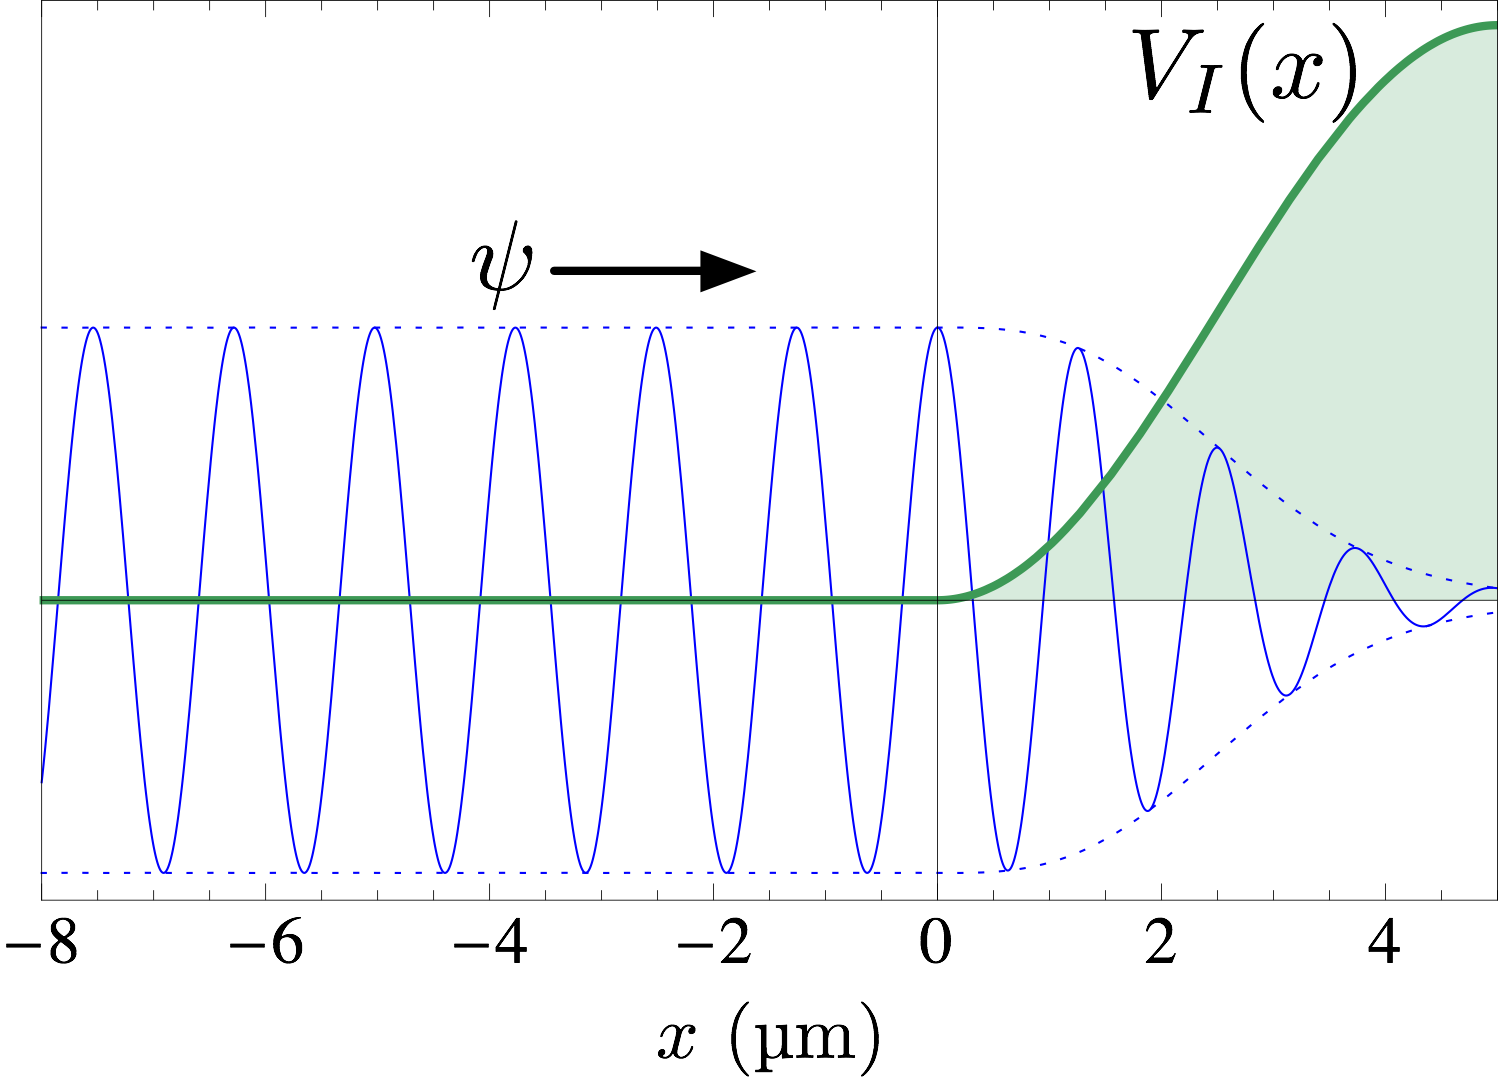
\includegraphics[width=8cm]{AbsorbingBoundarySchematic}
    \caption{
        \label{BackgroundTheory:AbsorbingBoundarySchematic}
        Schematic diagram illustrating the use of an absorbing boundary layer. A right-travelling wave is incident on the absorbing boundary layer which is given by the potential $V(x) = -i V_I(x)$. The wave is attenuated as it crosses the absorbing boundary layer.
    }
\end{figure}

An absorbing boundary layer of finite thickness can only be effective over a finite range of incident wavenumbers. Incident wavefunctions with large wavelengths (low wavenumbers) will be reflected from the absorbing boundary layer due to the rapid variation in the potential over a wavelength. Incident wavenumbers with very short wavelengths (high wavenumbers) will be transmitted through the absorbing boundary layer due to the finite amount of time spent in the absorbing boundary layer by any point on the phase-front.  Using this argument~\citet{Neuhasuer:1989} showed that the approximate range of wavenumbers over which an absorbing boundary layer will be effective is
\begin{align}
    \label{BackgroundTheory:AbsorbingBoundaryKEffectiveRange}
    \left( \frac{M \overline{V_I}}{\hbar^2 \Delta x}\right)^{\frac{1}{3}} \ll k \ll \frac{4 M \overline{V_I} \Delta x}{\hbar^2},
\end{align}
where $\overline{V_I}$ is a representative value of $V_I(x)$. The maximum and minimum limits for the wavenumber are respectively due to the requirements of negligible transmission and reflection. Although cast in terms of the wavenumber, \eqref{BackgroundTheory:AbsorbingBoundaryKEffectiveRange} is equivalent to (26) in~\citep{Neuhasuer:1989}. While not its purpose, \sectionref{MethodsAppendix:MomentumDensityFluxExampleCalculation} demonstrates how to calculate the reflection and transmission coefficients as a function of wavenumber for arbitrary absorbing boundary layers.

The use of absorbing boundary layers must be slightly modified for use in phase-space methods such as those discussed in \sectionref{BackgroundTheory:PhaseSpaceMethods}. In these cases simply adding an absorbing boundary layer to the potential would lead to unphysical results as the absorbing potential would not discriminate between real particles in a mode and the virtual particles which represent the fundamental vacuum fluctuations inherent in the field. An appropriate way of handling this problem is to add a position-dependent loss term to the master equation of the form
\begin{align}
    \label{BackgroundTheory:PhaseSpaceAbsorbingBoundaryLayer}
    \frac{d \hat{\rho}}{dt} &= \int d \vect{x}\, \frac{2}{\hbar}V_I(\vect{x})\mathcal{D}[\hat{\Psi}(\vect{x})]\hat{\rho},
\end{align}
where $\mathcal{D}$ is the usual decoherence superoperator. This master equation term leads to the same imaginary potential term in the equations of motion for the field operator with an additional noise term the for Truncated Wigner and Q function methods that restores the vacuum fluctuations that would otherwise be lost.

\parasep

In most of this thesis it is only the immediate vicinity of the BEC that is under consideration and absorbing boundary layers are used to restrict the computational domain to this region.  As the use of absorbing boundary layers is a technical issue not related to the underlying physics, they are not included in equations of motion given in this thesis but should be understood to be included when simulations are performed.  

While direct application of absorbing boundary layers permit the study of dynamics near the BEC, in \chapterref{TransverseProfile} the transverse profile of the atom laser a large distance from the BEC is considered.  In this case a different strategy must be used to avoid the $N_\text{pts} \propto t^3$ scaling discussed above.  Such a strategy is discussed in \sectionref{TransverseProfile:DropGP}.

\section{Spontaneous symmetry-breaking and all that}
\label{BackgroundTheory:SymmetryBreaking}

Quantum-mechanics is \emph{linear}. If my system is in the state $\displaystyle \hat{\rho} = \sum_i P_i \ketbra{\Psi_i}{\Psi_i}$, then I can simply consider the evolution of each of the $\displaystyle \rho_i = \ketbra{\Psi_i}{\Psi_i}$ \emph{individually} and then construct the weighted average for any expectation value that I'm interested in $\mean{\hat{O}} = \sum_i P_i \bra{\Psi_i}\hat{O}\ket{\Psi_i}$. Hence, the problem of `there is no mean field' is meaningless, as we can never measure the quantity $\mean{\hat{\Psi}}$, it is only ever number-conserving operators that are physically meaningful for atoms. Because of all this, the state $\hat{\rho} = \ketbra{\Psi}{\Psi}$ where $\ket{\Psi}$ is a coherent state is physically \emph{indistinguishable} from the state $\displaystyle \hat{\rho} = \frac{1}{2\pi}\int d\phi\, \ketbra{\Psi e^{i\phi}}{\Psi e^{i\phi}}$. Hence I can make my damned mean-field approximation if I want to. And I won't hear any complaints that it is `unphysical'. Some useful papers~\citep{Leggett:1991fj,Molmer:1997fr}

\section{Truncated Wigner}
\label{BackgroundTheory:TruncatedWigner}
We must talk about the initial state noise being interpreted as `virtual' particles. The exact number required due to the vacuum energy of the harmonic oscillator.
Operator correspondences must be described here.
\section{Rubidium}
\label{BackgroundTheory:Rubidium}
\section{Metastable helium}
\label{BackgroundTheory:Helium}

\begin{table}
    \centering
    \begin{tabular}{cc}
    \toprule
    Parameter & Value\\
    \midrule
    Quasimolecule $S=0$ scattering length & $a_{S=0}=\unit[9.46]{nm}$\\
    Quasimolecule $S=2$ scattering length & $a_{S=2}=\unit[7.51]{nm}$\\
    Penning ionisation rate & $\Kunpol = \unit[7.7\times 10^{-17}]{m\textsuperscript{3}}$\\
    \bottomrule
    \end{tabular}
    \caption{\label{BackgroundTheory:He*Parameters} Relevant parameters of metastable helium.}
\end{table}

\subsection{Penning ionisation}
\label{BackgroundTheory:PenningIonisation}

The primary attraction of creating Bose-Einstein condensates of metastable helium atoms is that their large internal energy ($\unit[20]{eV}$) enables single-atom detection with high spatial (\micro m) and temporal resolution (ns). However, this large internal energy can be released when two metastable helium atoms collide resulting in Penning ionisation (PI),
\begin{align}
    \label{BackgroundTheory:PenningIonisation}
    \text{He}^* + \text{He}^* & \rightarrow \left\{
        \begin{matrix}
            \text{He}^+ + \text{He} + e^-\\
            \text{He}_2^+ + e^-
        \end{matrix}\right.
\end{align}
While this process dominates for unpolarised cold samples such as magneto-optical traps~\citep{Bardou:1992}, it does not prohibit the formation of Bose-Einstein condensates as the process is suppressed by five orders of magnitude~\citep{Shlyapnikov:1994} in polarised samples.  This suppression is due to conservation of angular momentum. While the reactants each have a total angular momentum $s=1$, giving their combined total angular momentum as either $S=0$ or $S=2$ (assuming $s$-wave collisions), the products each have total angular momentum $s=\frac{1}{2}$ (in the case of $\text{He}^+$, $e^-$ and $\text{He}_2^+$) or $s=0$ (for $\text{He}$), giving the total angular momentum of the products as either $S=0$ or $S=1$. Hence spin polarised states having $S=2$, $m_S=\pm2$ cannot directly undergo the process \eqref{BackgroundTheory:PenningIonisation}.

In general as $S$ is conserved, any of the $S=2$ quasimolecule states will be prevented from directly undergoing Penning ionisation. As collisions with nonzero relative angular momentum can be neglected at BEC temperatures~\citep{Venturi:2000,Stas:2006kx} (due to the atoms having insufficient energy to penetrate the centrifugal barrier), it is only the $S=0$ quasimolecule state that undergoes Penning ionisation.

As derived in \sectionref{PenningIonisationAppendix:MasterEquation} the master equation term describing Penning ionisation is
\begin{align}
    \left.\frac{d \hat{\rho}}{dt}\right|_\text{PI} &= \frac{9}{2} \Kunpol \int d \vect{x}\, \mathcal{D}\left[ \hat{\Xi}_{S=0, m_S=0}\right] \hat{\rho},
\end{align}
where $\Kunpol = \unit[7.7\times 10^{-17}]{m\textsuperscript{3}s\textsuperscript{-1}}$ is the rate constant for the production of ions due to Penning ionisation in an unpolarised thermal sample at $\unit[1]{\micro K}$~\citep{Stas:2006kx}, and the $S=0$ quasimolecule state that undergoes Penning ionisation is given by
\begin{align}
    \hat{\Xi}_{S=0, m_S=0} &= \frac{1}{\sqrt{3}} \left( 2 \hat{\Psi}_1 \hat{\Psi}_{-1} - \hat{\Psi}_0 \hat{\Psi}_0\right).
\end{align}

\section{Pumping and (atom) lasers}
\label{BackgroundTheory:Lasers}
A brief overview of what gives a laser its properties. Refer to Wiseman's paper~\citep{Wiseman:1997ba} and compare the optical and atom lasers. Alternatives for the irreversibility / source are discussed in \chapterref{OpticalPumping,KineticTheory}.

There are two fundamental reasons making the pumping of an atom laser harder than pumping an optical laser is that the dispersion relation for potential reservoirs is not flat by comparison to the dispersion relation for atoms.  For an optical laser in the homogeneous broadening limit, \emph{all} atoms in the sample can contribute to gain.  Fundamentally this is because independent of what momentum the atom might have, it can still be stimulated to emit a photon into the lasing mode as the decay rates of the excited and/or ground atomic states are greater than any possible energy detuning in this process.  The second fundamental issue affecting atom lasers is that atom number is conserved.  It is therefore inescapable that there will be atoms in a (potentially) non-condensed source mode in the vicinity of the lasing mode.  Unless a Feschbach resonance is used to set the scattering-length of atomic interactions to zero, the atoms in the source mode will disrupt the phase stability of the lasing mode.

In \chapterref{OpticalPumping}, we attempt to solve the first problem by making the momentum distribution of source atoms sufficiently narrow that it can be guaranteed that every atom will be momentum-resonant with the pumping process at some point.  In \chapterref{KineticTheory}, we use atomic modes as the reservoir.  Although their dispersion relation cannot be flat with respect to that of the atoms in the source mode, it is at least far more comparable than that of light (which is used in \chapterref{OpticalPumping}).

Ideally we should pump an atom laser using something with a flat dispersion relation.  One possibility that comes to mind is the phonon.  However it is necessary that the reservoir is essentially a pure vacuum.  Phonons produced in a condensate cannot escape the system unless the system is in contact with other atoms.  If these other atoms are thermal, than it will have its own phonons which will propagate into the condensate.  If the condensate is not in physical contact with anything, then the phonons cannot leave the system: there is no evaporation process for phonons.

Stolen from \citep{Ballagh:2000oq}:
Despite the parallels with optical laser theory, the fundamental differences between photons and atoms remain important. They arise principally because atoms have rest mass, and because they interact with each other. Unlike photons, atoms cannot be created or destroyed, rather they are transferred into the laser mode from some other mode. The interactions produce phase dynamics, which degrades the coherence of the atom laser, and self repulsion which spreads the output beam and limits the possible focussing. Even when these interactions are neglected, atoms have dispersive propagation in vacuum.
